\ylDisplay{Tsunami} % Ülesande nimi
{Jaan Kalda} % Autor
{lõppvoor} % Voor
{2005} % Aasta
{G 6} % Ülesande nr.
{6} % Raskustase
{
% Teema: Kinemaatika
\ifStatement
\begin{wrapfigure}[10]{r}{0.45\textwidth}
	\begin{center}
		\vspace{-20pt}
		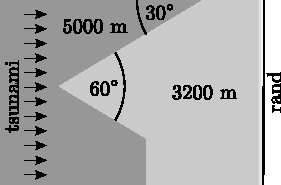
\includegraphics[width=\linewidth]{2005-v3g-06-yl}
	\end{center}
\end{wrapfigure}

Joonisel on ülaltvaates toodud ookeanipõhja sügavus kodeeritud halltoonidega: tumedam hall vastab sügavamale, heledam hall madalamale veele. Ookeanipõhjas on astang, kus $h_1 = \SI{5000}{m}$ sügavune vesi läheb $h_2 = \SI{3200}{m}$ sügavuseks; ranna lähedal toimub madaldumine väga kiiresti. Rannale läheneb tsunami nii, nagu näidatud joonisel. Tsunami liikumiskiirus $v = \sqrt{gh}$, kus $g = \SI{9,8}{m/s^2}$ ja $h$ tähistab vee sügavust. Millisesse ranna punkti jõuab kõige kõrgem laine? Põhjendage vastust.
\fi


\ifHint
Laine levik toimub geomeetrilise optika seaduste kohaselt. Kehtib $\sin \alpha_{1}/\sin \alpha_{2}=v_{1}/v_{2}$, kus $v_i$ ja $\alpha_i$ on vastavalt keskkonna $i\in \{1, 2\}$ laine leviku kiirus ja langemisnurk eralduspinna normaali suhtes.
\fi


\ifSolution
Laine levik toimub geomeetrilise optika seaduste kohaselt: astangu juures on laine langemisnurga ja murdumisnurga suhe
\[
\frac{\sin \alpha_{1}}{\sin \alpha_{2}}=\frac{v_{1}}{v_{2}}=\frac{\sqrt{g h_{1}}}{\sqrt{g h_{2}}}=\sqrt{\frac{h_{1}}{h_{2}}} \quad\Rightarrow\quad \alpha_{2}=\arcsin \left(\sin \alpha_{1} \sqrt{\frac{h_{2}}{h_{1}}}\right).
\]
Seal astangu osas, kus langemisnurk on \SI{0}{\degree}, murdumist ei toimu. Seal aga, kus $\alpha_1 = \SI{60}{\degree}$, on murdumisnurk
\[
\alpha_{2}=\arcsin \left(\sin \SI{60}{\degree} \sqrt{\frac{3200}{5000}}\right) \approx \SI{44}{\degree}.
\]
Seega kaldub laine esialgsest levimissuunast kõrvale nurga $\beta = \alpha_1 -\alpha_2 = \SI{16}{\degree}$ võrra. Niisiis jõuab rannalõigule $AC$ kaks lainet ning rannalõigule $DE$ ei jõua üldse lainet. Punkti $B$ jõuavad mõlemad lained üheaegselt (sümmeetria tõttu) ning seal ongi laine kõige kõrgem.

\begin{center}
	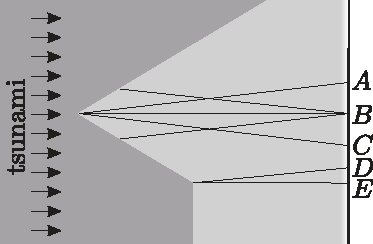
\includegraphics[width=0.6\linewidth]{2005-v3g-06-lah}
\end{center}
\fi
}